

\providecommand{\keywords}[1]{\textbf{\textit{Keywords:}} #1}
\section{Houdini basics}

word\footnote{Explanation of the word.} that
ddjword\footnote{Explanation of the word.} that
jord\footnote{Explanation of the word.} that

You can find the source code on GitHub: \url{https://github.com/your-username/your-repository}.



\begin{figure}[H] 
    \centering
    \begin{subfigure}[b]{0.49\textwidth}
        \centering
        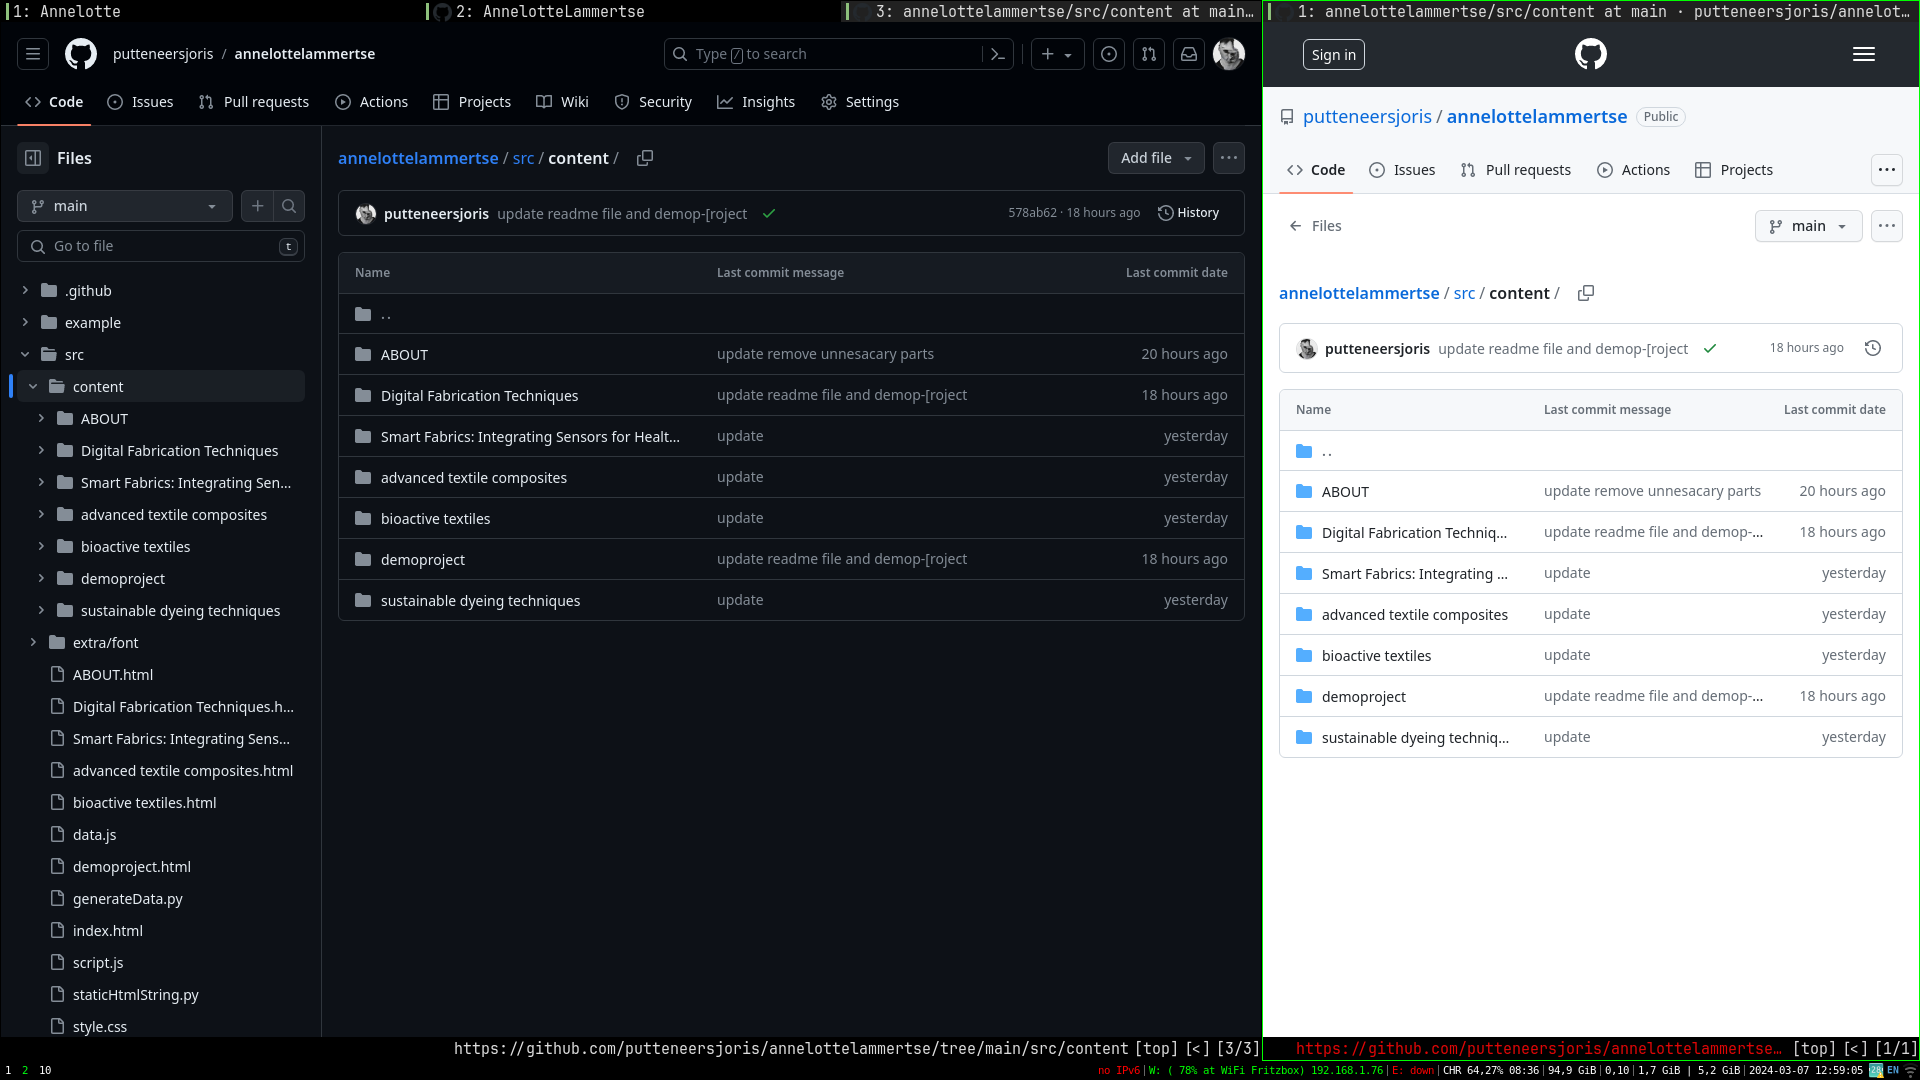
\includegraphics[width=1\textwidth]{sections/assignment_1/1.png}
        \caption{digital signal}
    \end{subfigure}
    \hfill
    \begin{subfigure}[b]{0.49\textwidth}
        \centering
        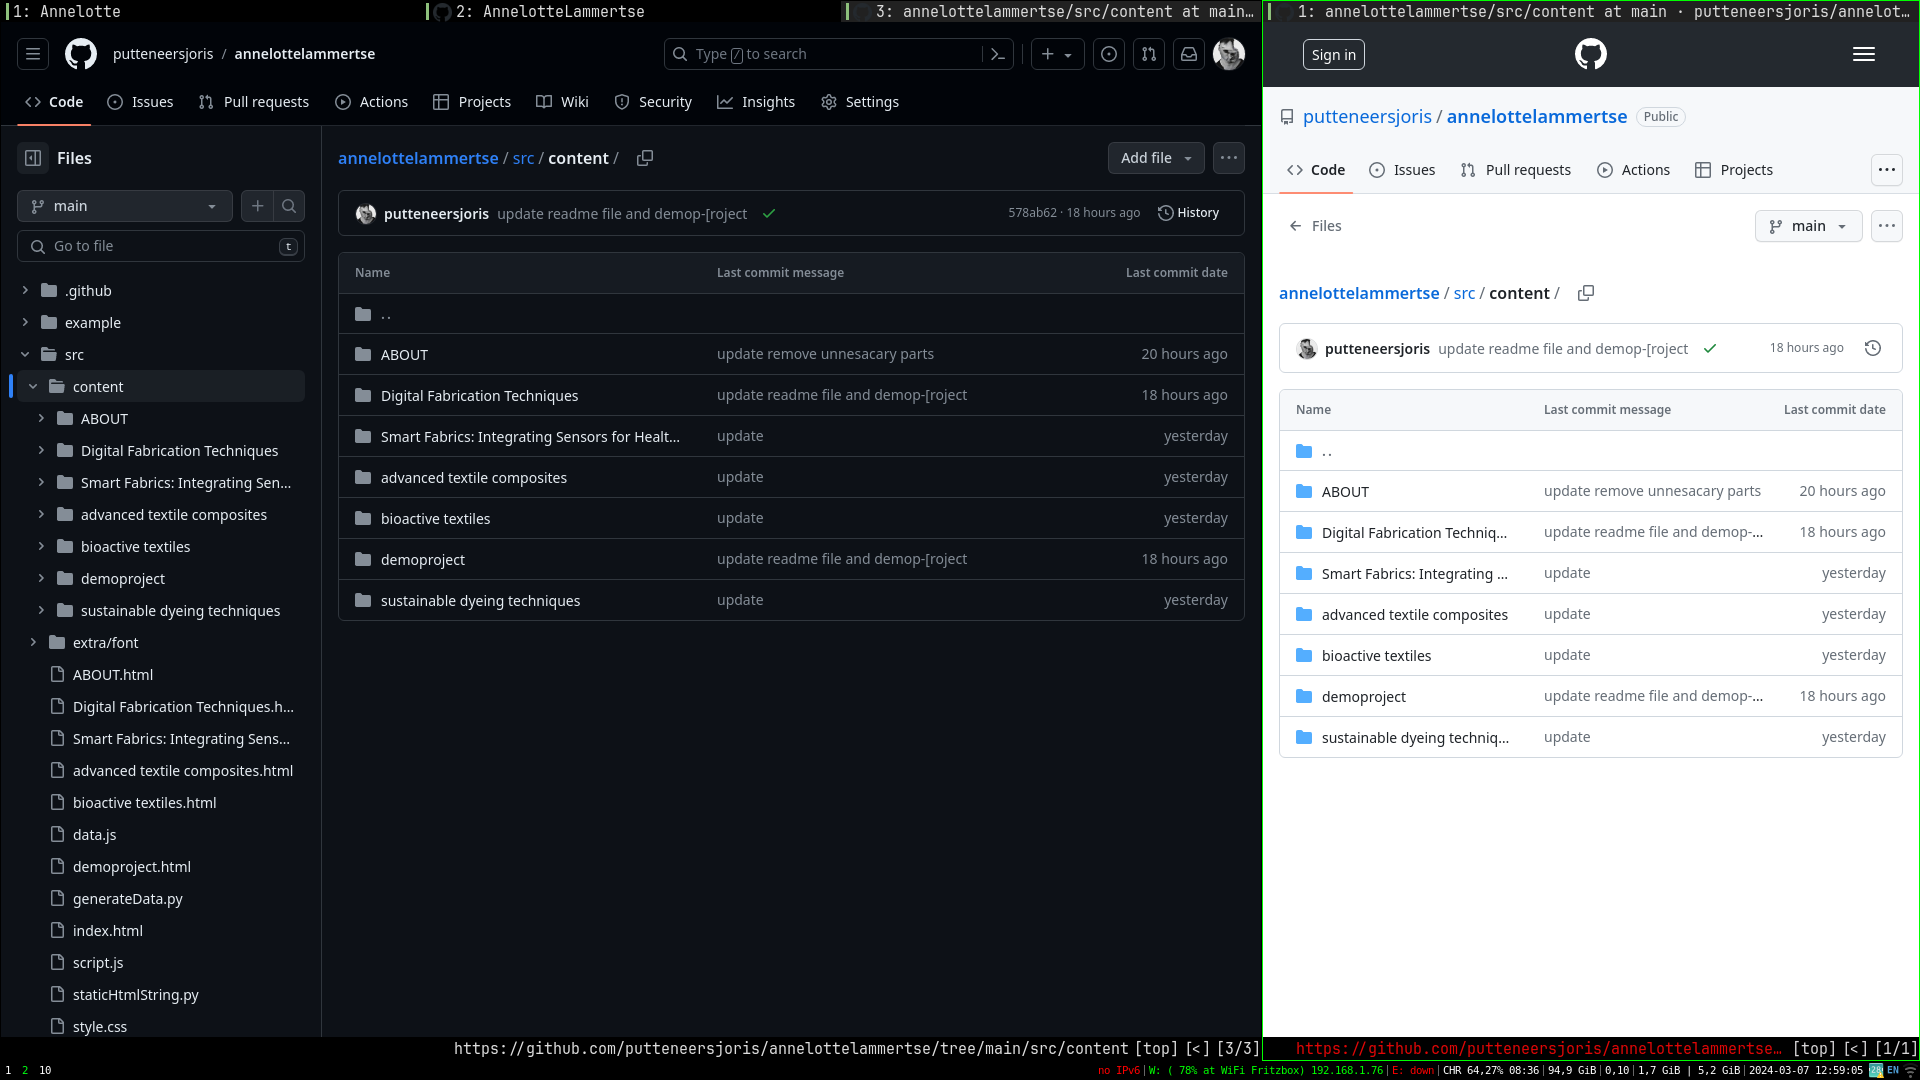
\includegraphics[width=1\textwidth]{sections/assignment_1/1.png}
        \caption{analog signal}
    \end{subfigure}
    \caption{data visualization.}
\end{figure}


% Define \keywords command to store keywords

\keywords{keyword1, keyword2, keyword3}









\begin{figure}[H] 
    \centering
    \begin{subfigure}[b]{0.45\textwidth}
        \centering
        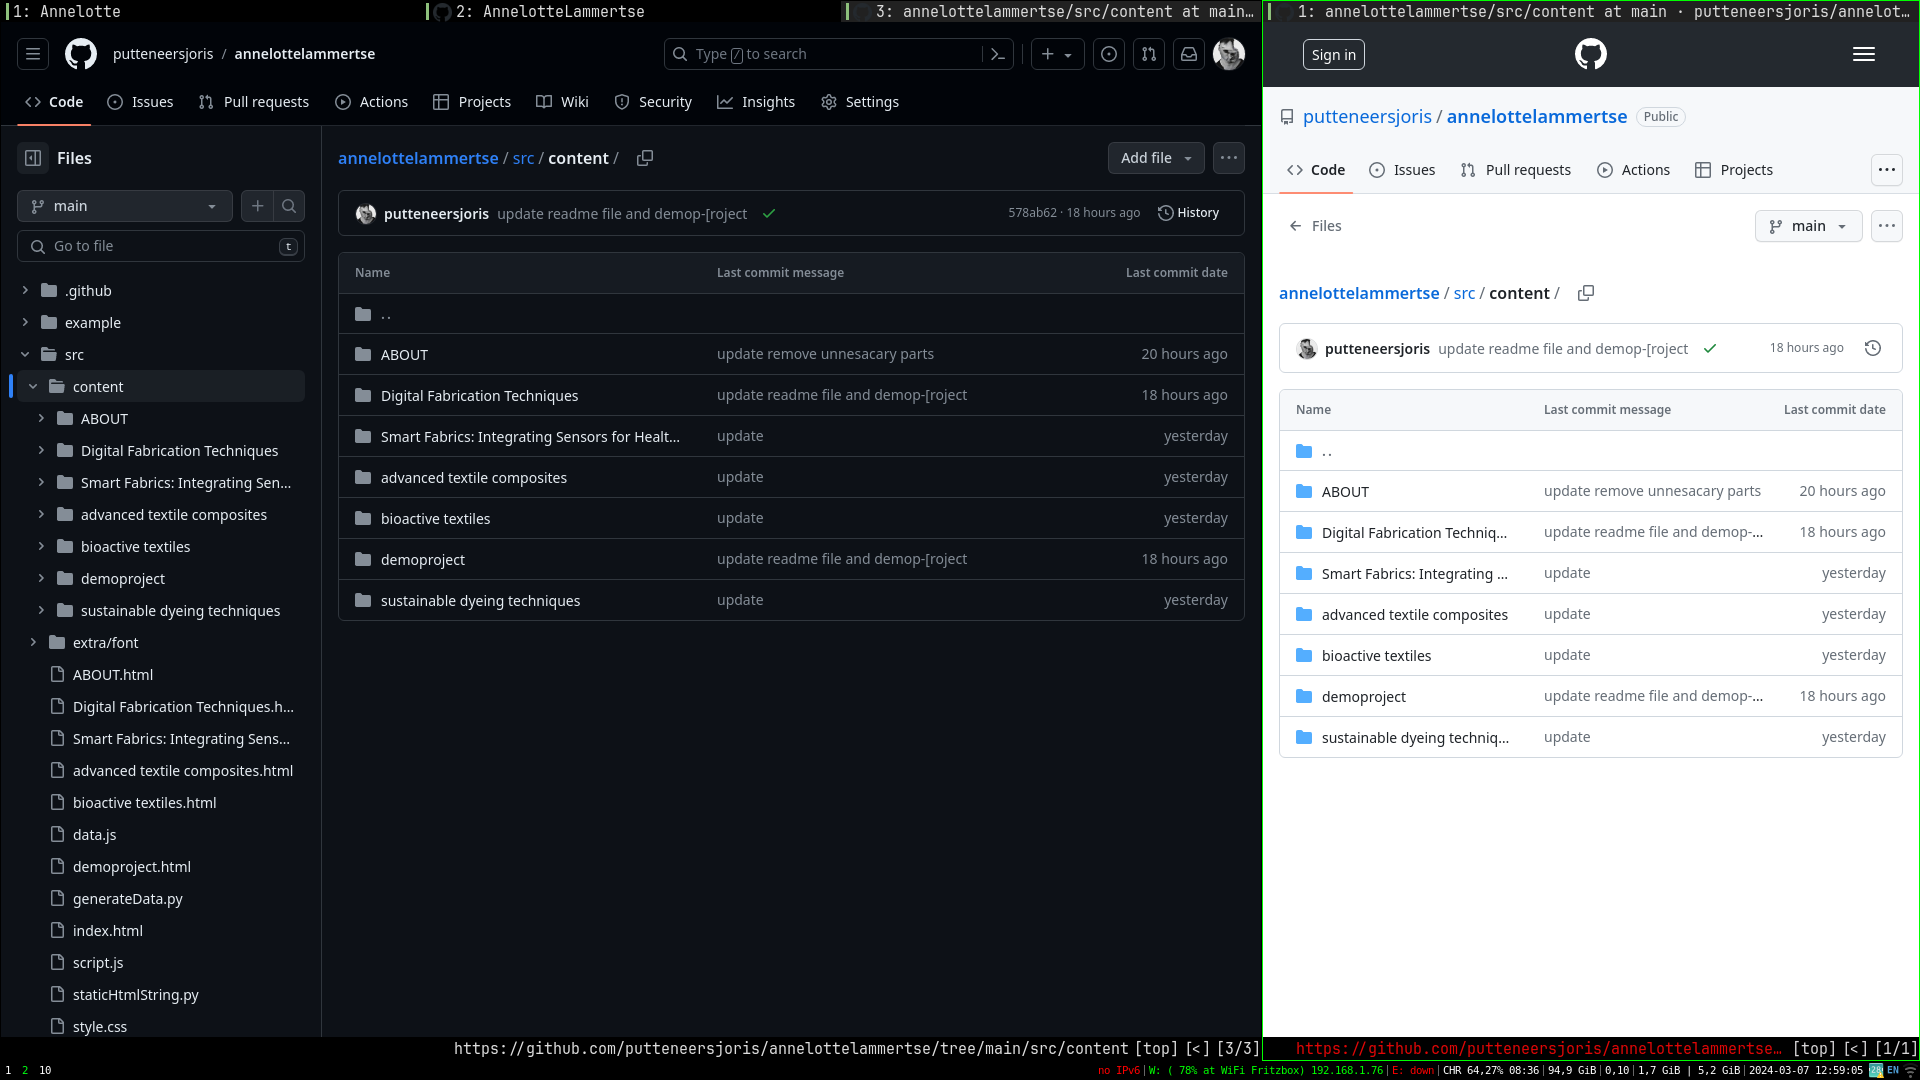
\includegraphics[width=1\textwidth]{sections/assignment_1/1.png}
        \caption{Digital signal}
    \end{subfigure}
    \hfill
    \begin{subfigure}[b]{0.45\textwidth}
        Some text describing the image goes here.

        \caption{Digital signal}
    \end{subfigure}
    \caption{Data visualization.}
    \label{fig:data_vis}
\end{figure}



